
\section{Latent-Function Video Diffusion}
\label{sec:method}

LFVD generates a shared latent representation that supports videos at
continuous control values. We first train a family encoder and a query
decoder using videos observed at different controls. We then train a Video
DiT to generate the shared representation. At inference, the same generated
representation supports multiple video queries. Figure~\ref{fig:architecture}
illustrates the two training stages and inference process.

\begin{figure*}[t]
\centering
\begin{subfigure}[t]{\textwidth}
  \centering
  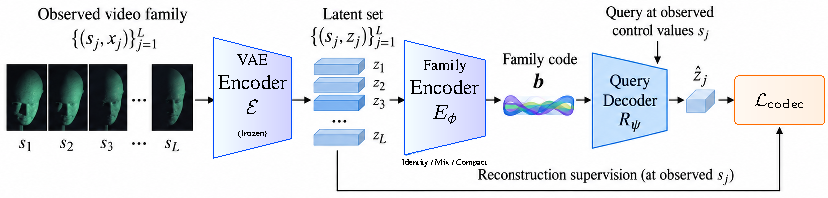
\includegraphics[width=\linewidth]{figures/fig2a_codec_training.pdf}
  \caption{Learning the family encoder and query decoder from observed videos.}
\end{subfigure}
\vspace{2pt}
\begin{subfigure}[t]{\textwidth}
  \centering
  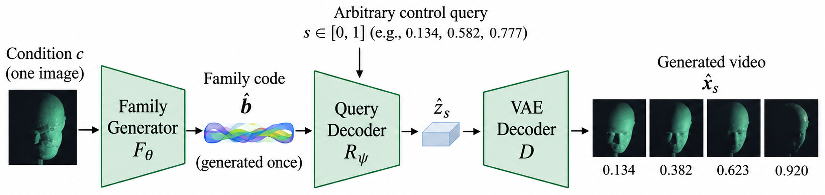
\includegraphics[width=\linewidth]{figures/fig2b_inference.pdf}
  \caption{Generating one shared representation and querying multiple videos.}
\end{subfigure}
\caption{\textbf{LFVD training and inference.} (a) A frozen video VAE
encodes the observed videos. The family encoder and query decoder learn a
shared latent representation through reconstruction. We then freeze these
components and train a Video DiT with flow matching. (b) At inference, the
Video DiT samples the non-reference portion of one shared representation,
while the reference latent remains fixed. The query decoder and frozen VAE
produce videos at requested control values without further denoising.}
\label{fig:architecture}
\end{figure*}

\subsection{Conditional Videos and Latent Functions}
\label{sec:formulation}

Let $c$ denote the shared input condition, including a reference image and
text, and let $s\in\mathcal S=[0,1]$ be a continuous control value. We write
$x_s$ for the video at control value $s$. A frozen video VAE consists of an
encoder $\mathcal E_{\mathrm{VAE}}$ and a decoder $\mathcal D_{\mathrm{VAE}}$.
We denote its video latent by $z_s=\mathcal E_{\mathrm{VAE}}(x_s)$. Let
$C$, $T_z$, $H$, and $W$ denote the channel, temporal, height, and width
dimensions of the \emph{VAE latent}, respectively. Thus,
$z_s\in\mathbb R^{C\times T_z\times H\times W}$; $H$ and $W$ refer to
latent spatial dimensions, not the resolution of the original video.

For pointwise generation, let $G_{\theta_{\mathrm{PW}}}$ be a conditional
diffusion sampler with parameters $\theta_{\mathrm{PW}}$. We use
$\varepsilon$ for its initial Gaussian noise, $\hat z_s$ for the generated
video latent, and $\hat x_s$ for the decoded video. Pointwise generation is
\begin{equation}
    \hat z_s=G_{\theta_{\mathrm{PW}}}(c,s,\varepsilon),\qquad
    \hat x_s=\mathcal D_{\mathrm{VAE}}(\hat z_s).
    \label{eq:baseline_generation}
\end{equation}
The sampler performs a complete denoising process for each requested control
value. LFVD instead uses a shared latent representation $\mathbf b$ and a
query decoder $R_\psi$, parameterized by $\psi$, to reconstruct an individual
video latent. Let $\mathcal Z_{\mathbf b}$ denote the resulting mapping from
control values to video latents:
\begin{equation}
\begin{aligned}
    \mathcal Z_{\mathbf b}:\mathcal S
      &\rightarrow \mathbb R^{C\times T_z\times H\times W},\\
    \mathcal Z_{\mathbf b}(s)&=R_\psi(\mathbf b,s).
\end{aligned}
    \label{eq:latent_function_definition}
\end{equation}
A single representation therefore provides a video latent for each
requested control value.

\subsection{Learning a Family Representation}
\label{sec:codec}

For each shared condition $c$, let $L$ denote the number of observed videos
and let $\ell\in\{1,\ldots,L\}$ index their control values $s_\ell$. We
write $z_\ell=\mathcal E_{\mathrm{VAE}}(x_{s_\ell})$ for the corresponding
latents and define the training family as
$\mathcal F_c=\{(s_\ell,x_{s_\ell})\}_{\ell=1}^{L}$. We divide each video
latent along the temporal dimension into a shared reference frame
$z_{\mathrm{shared}}\in\mathbb R^{C\times1\times H\times W}$ and the
remaining $T_z-1$ frames $z_{\ell,\mathrm{rest}}$, giving
$z_\ell=[z_{\mathrm{shared}},z_{\ell,\mathrm{rest}}]$. The total number of
non-reference latent frames across the observed videos is
$J=L(T_z-1)$.

Let $E_\phi$ denote the family encoder, with parameters $\phi$ when learned.
It combines the non-reference video latents into an encoded representation
$\mathbf b_{0,\mathrm{rest}}$ containing $J'$ latent frames. Our encoder
preserves the VAE latent channel and spatial dimensions $C$, $H$, and $W$,
and transforms only the latent-time dimension. Therefore,
$\mathbf b_{0,\mathrm{rest}}\in
\mathbb R^{C\times J'\times H\times W}$. We concatenate this encoded
representation with the unchanged reference frame to obtain the complete
family code $\mathbf b_0$:
\begin{equation}
\begin{aligned}
    \mathbf b_{0,\mathrm{rest}}
      &=E_\phi\!\left(\{(s_\ell,z_{\ell,\mathrm{rest}})\}_{\ell=1}^{L}\right),\\
    \mathbf b_0&=[z_{\mathrm{shared}},\mathbf b_{0,\mathrm{rest}}].
\end{aligned}
\label{eq:family_encoding}
\end{equation}
The family encoder can be fixed or learned.



\paragraph{Family encoder variants.}
We implement the family encoder $E_\phi$ in
Eq.~\ref{eq:family_encoding} using a temporal projection.
Let $\operatorname{Emb}_\phi(s)\in\mathbb R^C$ denote an optional
control embedding, $\lambda$ its scale, and
$P_\phi\in\mathbb R^{J'\times J}$ a temporal projection.
The embedding is broadcast over time and space, and the video
latents are concatenated in control-value order:
\begin{equation}
    \mathbf b_{0,\mathrm{rest}}
    =P_\phi\operatorname{Concat}_{\ell,\mathrm{time}}
    \left(z_{\ell,\mathrm{rest}}
    +\lambda\operatorname{Emb}_\phi(s_\ell)\right).
    \label{eq:family_mixer}
\end{equation}
The three encoder variants are defined by
\[
\begin{aligned}
    \text{Identity:}\quad &J'=J,\; P_\phi=I,\; \lambda=0,\\
    \text{Mix:}\quad &J'=J,\; P_\phi\in\mathbb R^{J\times J},\\
    \text{Compact:}\quad &J'<J,\; P_\phi\in\mathbb R^{J'\times J}.
\end{aligned}
\]
Here, $I$ is the identity matrix. Identity directly concatenates
the observed latents, Mix learns temporal mixing and control
embeddings, and Compact reduces the representation length.




\paragraph{Continuous query decoder.}
Given the family code $\mathbf b_0$ and a control value $s$,
the query decoder $R_\psi$ uses an $s$-conditioned neural network
to generate a temporal projection $A_\psi(s)$ and a bias
$\beta_\psi(s)$. Their dimensions and the decoding process are
\begin{equation}
\begin{aligned}
    A_\psi(s)
    &\in\mathbb R^{(T_z-1)\times J'},\\
    \beta_\psi(s)
    &\in\mathbb R^{C\times(T_z-1)},\\
    \hat z_{s,\mathrm{rest}}
    &=A_\psi(s)\mathbf b_{0,\mathrm{rest}}+\beta_\psi(s),\\
    R_\psi(\mathbf b_0,s)
    &=[z_{\mathrm{shared}},\hat z_{s,\mathrm{rest}}].
\end{aligned}
\label{eq:direct_query}
\end{equation}


\paragraph{Representation capacity.}
Identity and Mix both use $J'=J$. On a fixed grid of observed control
values, the query decoder can absorb an invertible temporal projection
and the control-embedding offsets. These variants therefore have the
same nominal reconstruction capacity when the Mix projection is
invertible, although they can produce different code distributions for
diffusion training. Compact reduces $J'$ and introduces a
compression--fidelity trade-off. We compare these effects in
Sec.~\ref{sec:encoder_ablation}.

\subsection{Diffusion over the Family Code}
\label{sec:learning}

After codec training, we freeze $E_\phi$ and $R_\psi$ and encode each
training family into a clean code $\mathbf b_0$. Let $\theta$ denote the
trainable Video DiT parameters. The model learns the conditional
distribution of family codes using standard flow
matching~\cite{lipman2023flow}.

Let $t\in[0,1]$ denote the normalized flow-matching noise level, and let
$\varepsilon$ be a Gaussian-noise draw with the same shape as
$\mathbf b_{0,\mathrm{rest}}$. We denote the noisy family code by
$\mathbf b_t$ and the target velocity of its non-reference portion by
$\mathbf v_{\mathrm{target}}$. The reference frame $z_{\mathrm{shared}}$
remains fixed, while the non-reference portion is interpolated between
its clean value and noise:
\begin{equation}
\begin{aligned}
    \mathbf b_t&=[z_{\mathrm{shared}},
       (1-t)\mathbf b_{0,\mathrm{rest}}+t\varepsilon],\\
    \mathbf v_{\mathrm{target}}&=\varepsilon-\mathbf b_{0,\mathrm{rest}}.
\end{aligned}
\label{eq:lfvd_forward}
\end{equation}
Let $\mathbf v_{\theta,\mathrm{rest}}$ denote the Video DiT's predicted
velocity for the non-reference portion, and let $w(t)$ denote the loss
weight defined by the pretrained scheduler. We write
$\mathcal L_{\mathrm{FM}}$ for the flow-matching loss and
$\|\cdot\|_2^2$ for squared error over the predicted elements. The
expectation covers training families, sampled noise levels, and Gaussian
noise. We minimize
\begin{equation}
    \mathcal L_{\mathrm{FM}}=
    \mathbb E\left[w(t)
    \|\mathbf v_{\theta,\mathrm{rest}}(\mathbf b_t,t,c)
      -\mathbf v_{\mathrm{target}}\|_2^2\right].
    \label{eq:lfvd_objective}
\end{equation}

At inference, let $F_\theta$ denote the complete sampling process
obtained by integrating the trained velocity predictor
$\mathbf v_{\theta,\mathrm{rest}}$. We use $\varepsilon$ again for an
independent Gaussian-noise draw, now with the shape of the family-code
non-reference portion. The sampler keeps $z_{\mathrm{shared}}$ fixed and
produces a family code $\hat{\mathbf b}$. Let $\hat x_s$ denote the video
at the requested control $s$. Generation follows
\begin{equation}
\begin{aligned}
    \hat{\mathbf b}&=F_\theta(c,\varepsilon),\\
    \hat x_s&=\mathcal D_{\mathrm{VAE}}
       \!\left(R_\psi(\hat{\mathbf b},s)\right).
\end{aligned}
\label{eq:lfvd_generation}
\end{equation}
The requested control value enters only the query decoder. Once the family
code has been sampled, each additional video requires a query-decoder
and VAE-decoder evaluation. 



\subsection{Multi-Query Generation Cost}
\label{sec:query}

The computational cost of LFVD depends on the family-code length
$J'$ and the number of requested videos $M$.
Let $\mathcal C_{\mathrm{diff}}(n)$ denote the cost of diffusion
sampling with $n$ latent frames, keeping the backbone, spatial
dimensions, and sampling steps fixed.
Let $\mathcal C_D$ denote the cost of one VAE decoding and
$\mathcal C_R(J')$ the cost of querying a family code of length
$1+J'$.

The query cost includes generating $A_\psi(s)$ and $\beta_\psi(s)$
and applying the temporal projection.
Let $\mathcal C_{\mathrm{param}}(J')$ denote the cost of generating
these projection parameters. Counting each multiply--accumulate
as two operations, the query cost is approximately
\begin{equation}
    \mathcal C_R(J')
    \approx \mathcal C_{\mathrm{param}}(J')
    +CHW(T_z-1)(2J'+1).
    \label{eq:query_cost}
\end{equation}

The total costs of pointwise generation
and LFVD for $M$ videos are
\begin{equation}
\begin{aligned}
    \mathcal C_{\mathrm{PW}}(M)
    &=M\mathcal C_D+M\mathcal C_{\mathrm{diff}}(T_z),\\
    \mathcal C_{\mathrm{LFVD}}(M)
    &=M\mathcal C_D+\mathcal C_{\mathrm{diff}}(1+J')\\
    &\quad+M\mathcal C_R(J').
\end{aligned}
\label{eq:generation_cost}
\end{equation}
Both methods require $M$ VAE decodings. The difference lies in
the repeated diffusion cost of pointwise generation and the
single diffusion cost followed by queries in LFVD.

Since the VAE costs cancel, LFVD becomes more efficient when
\begin{equation}
    M>
    \frac{\mathcal C_{\mathrm{diff}}(1+J')}
    {\mathcal C_{\mathrm{diff}}(T_z)-\mathcal C_R(J')},
    \label{eq:cost_crossover}
\end{equation}
provided that
$\mathcal C_{\mathrm{diff}}(T_z)>\mathcal C_R(J')$.
This condition gives the minimum query count needed to amortize
the family-generation cost under the sequential cost model.
We evaluate the actual crossover, including batched pointwise
generation, in Sec.~\ref{sec:cost}.
